\documentclass[1p]{elsarticle_modified}
%\bibliographystyle{elsarticle-num}

%\usepackage[colorlinks]{hyperref}
%\usepackage{abbrmath_seonhwa} %\Abb, \Ascr, \Acal ,\Abf, \Afrak
\usepackage{amsfonts}
\usepackage{amssymb}
\usepackage{amsmath}
\usepackage{amsthm}
\usepackage{scalefnt}
\usepackage{amsbsy}
\usepackage{kotex}
\usepackage{caption}
\usepackage{subfig}
\usepackage{color}
\usepackage{graphicx}
\usepackage{xcolor} %% white, black, red, green, blue, cyan, magenta, yellow
\usepackage{float}
\usepackage{setspace}
\usepackage{hyperref}

\usepackage{tikz}
\usetikzlibrary{arrows}

\usepackage{multirow}
\usepackage{array} % fixed length table
\usepackage{hhline}

%%%%%%%%%%%%%%%%%%%%%
\makeatletter
\renewcommand*\env@matrix[1][\arraystretch]{%
	\edef\arraystretch{#1}%
	\hskip -\arraycolsep
	\let\@ifnextchar\new@ifnextchar
	\array{*\c@MaxMatrixCols c}}
\makeatother %https://tex.stackexchange.com/questions/14071/how-can-i-increase-the-line-spacing-in-a-matrix
%%%%%%%%%%%%%%%

\usepackage[normalem]{ulem}

\newcommand{\msout}[1]{\ifmmode\text{\sout{\ensuremath{#1}}}\else\sout{#1}\fi}
%SOURCE: \msout is \stkout macro in https://tex.stackexchange.com/questions/20609/strikeout-in-math-mode

\newcommand{\cancel}[1]{
	\ifmmode
	{\color{red}\msout{#1}}
	\else
	{\color{red}\sout{#1}}
	\fi
}

\newcommand{\add}[1]{
	{\color{blue}\uwave{#1}}
}

\newcommand{\replace}[2]{
	\ifmmode
	{\color{red}\msout{#1}}{\color{blue}\uwave{#2}}
	\else
	{\color{red}\sout{#1}}{\color{blue}\uwave{#2}}
	\fi
}

\newcommand{\Sol}{\mathcal{S}} %segment
\newcommand{\D}{D} %diagram
\newcommand{\A}{\mathcal{A}} %arc


%%%%%%%%%%%%%%%%%%%%%%%%%%%%%5 test

\def\sl{\operatorname{\textup{SL}}(2,\Cbb)}
\def\psl{\operatorname{\textup{PSL}}(2,\Cbb)}
\def\quan{\mkern 1mu \triangleright \mkern 1mu}

\theoremstyle{definition}
\newtheorem{thm}{Theorem}[section]
\newtheorem{prop}[thm]{Proposition}
\newtheorem{lem}[thm]{Lemma}
\newtheorem{ques}[thm]{Question}
\newtheorem{cor}[thm]{Corollary}
\newtheorem{defn}[thm]{Definition}
\newtheorem{exam}[thm]{Example}
\newtheorem{rmk}[thm]{Remark}
\newtheorem{alg}[thm]{Algorithm}

\newcommand{\I}{\sqrt{-1}}
\begin{document}

%\begin{frontmatter}
%
%\title{Boundary parabolic representations of knots up to 8 crossings}
%
%%% Group authors per affiliation:
%\author{Yunhi Cho} 
%\address{Department of Mathematics, University of Seoul, Seoul, Korea}
%\ead{yhcho@uos.ac.kr}
%
%
%\author{Seonhwa Kim} %\fnref{s_kim}}
%\address{Center for Geometry and Physics, Institute for Basic Science, Pohang, 37673, Korea}
%\ead{ryeona17@ibs.re.kr}
%
%\author{Hyuk Kim}
%\address{Department of Mathematical Sciences, Seoul National University, Seoul 08826, Korea}
%\ead{hyukkim@snu.ac.kr}
%
%\author{Seokbeom Yoon}
%\address{Department of Mathematical Sciences, Seoul National University, Seoul, 08826,  Korea}
%\ead{sbyoon15@snu.ac.kr}
%
%\begin{abstract}
%We find all boundary parabolic representation of knots up to 8 crossings.
%
%\end{abstract}
%\begin{keyword}
%    \MSC[2010] 57M25 
%\end{keyword}
%
%\end{frontmatter}

%\linenumbers
%\tableofcontents
%
\newcommand\colored[1]{\textcolor{white}{\rule[-0.35ex]{0.8em}{1.4ex}}\kern-0.8em\color{red} #1}%
%\newcommand\colored[1]{\textcolor{white}{ #1}\kern-2.17ex	\textcolor{white}{ #1}\kern-1.81ex	\textcolor{white}{ #1}\kern-2.15ex\color{red}#1	}

{\Large $\underline{12a_{0577}~(K12a_{0577})}$}

\setlength{\tabcolsep}{10pt}
\renewcommand{\arraystretch}{1.6}
\vspace{1cm}\begin{tabular}{m{100pt}>{\centering\arraybackslash}m{274pt}}
\multirow{5}{120pt}{
	\centering
	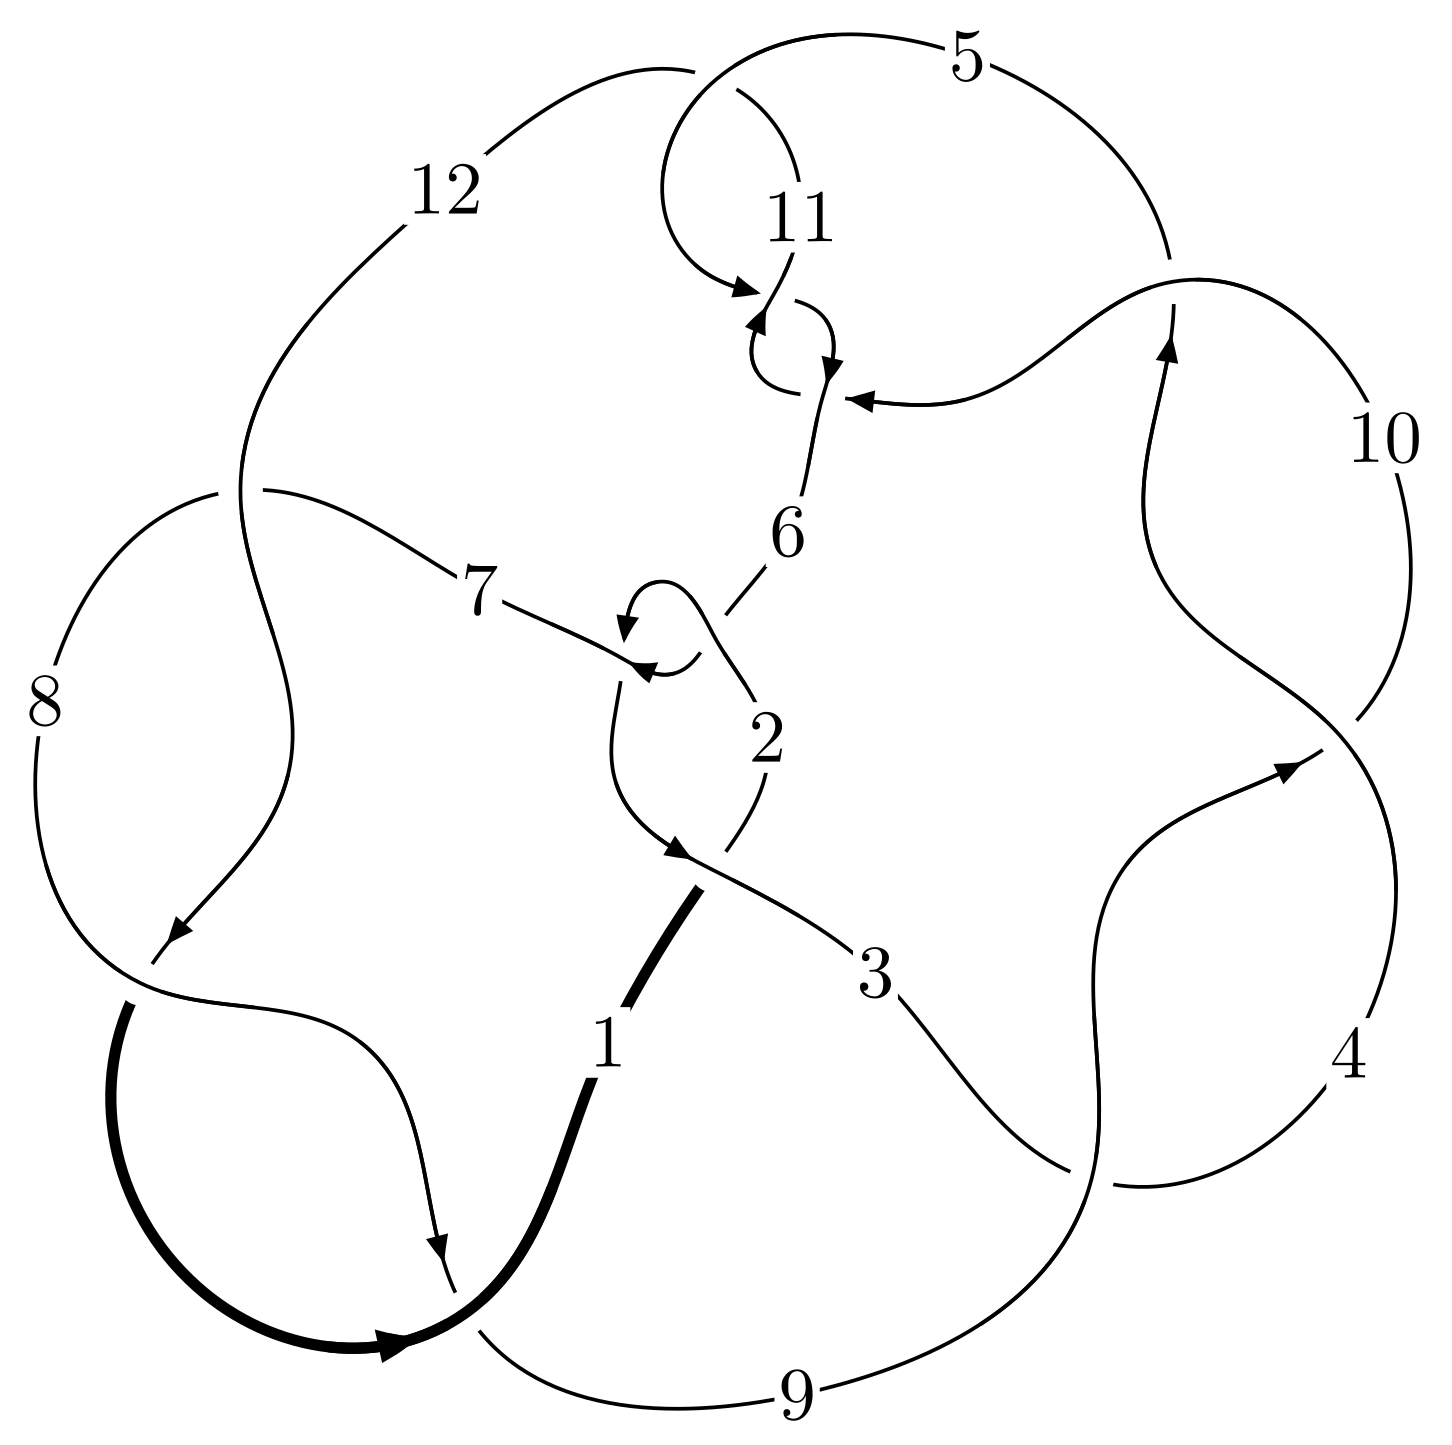
\includegraphics[width=112pt]{../../../GIT/diagram.site/Diagrams/png/1378_12a_0577.png}\\
\ \ \ A knot diagram\footnotemark}&
\allowdisplaybreaks
\textbf{Linearized knot diagam} \\
\cline{2-2}
 &
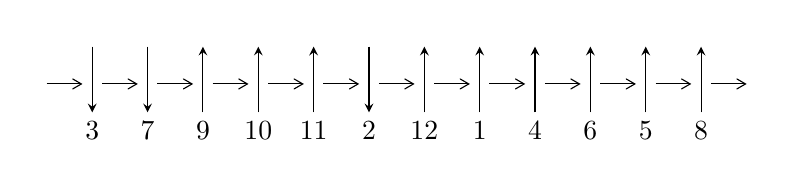
\begin{tikzpicture}[x=20pt, y=17pt]
	% nodes
	\node (C0) at (0, 0) {};
	\node (C1) at (1, 0) {};
	\node (C1U) at (1, +1) {};
	\node (C1D) at (1, -1) {3};

	\node (C2) at (2, 0) {};
	\node (C2U) at (2, +1) {};
	\node (C2D) at (2, -1) {7};

	\node (C3) at (3, 0) {};
	\node (C3U) at (3, +1) {};
	\node (C3D) at (3, -1) {9};

	\node (C4) at (4, 0) {};
	\node (C4U) at (4, +1) {};
	\node (C4D) at (4, -1) {10};

	\node (C5) at (5, 0) {};
	\node (C5U) at (5, +1) {};
	\node (C5D) at (5, -1) {11};

	\node (C6) at (6, 0) {};
	\node (C6U) at (6, +1) {};
	\node (C6D) at (6, -1) {2};

	\node (C7) at (7, 0) {};
	\node (C7U) at (7, +1) {};
	\node (C7D) at (7, -1) {12};

	\node (C8) at (8, 0) {};
	\node (C8U) at (8, +1) {};
	\node (C8D) at (8, -1) {1};

	\node (C9) at (9, 0) {};
	\node (C9U) at (9, +1) {};
	\node (C9D) at (9, -1) {4};

	\node (C10) at (10, 0) {};
	\node (C10U) at (10, +1) {};
	\node (C10D) at (10, -1) {6};

	\node (C11) at (11, 0) {};
	\node (C11U) at (11, +1) {};
	\node (C11D) at (11, -1) {5};

	\node (C12) at (12, 0) {};
	\node (C12U) at (12, +1) {};
	\node (C12D) at (12, -1) {8};
	\node (C13) at (13, 0) {};

	% arrows
	\draw[->,>={angle 60}]
	(C0) edge (C1) (C1) edge (C2) (C2) edge (C3) (C3) edge (C4) (C4) edge (C5) (C5) edge (C6) (C6) edge (C7) (C7) edge (C8) (C8) edge (C9) (C9) edge (C10) (C10) edge (C11) (C11) edge (C12) (C12) edge (C13) ;	\draw[->,>=stealth]
	(C1U) edge (C1D) (C2U) edge (C2D) (C3D) edge (C3U) (C4D) edge (C4U) (C5D) edge (C5U) (C6U) edge (C6D) (C7D) edge (C7U) (C8D) edge (C8U) (C9D) edge (C9U) (C10D) edge (C10U) (C11D) edge (C11U) (C12D) edge (C12U) ;
	\end{tikzpicture} \\
\hhline{~~} \\& 
\textbf{Solving Sequence} \\ \cline{2-2} 
 &
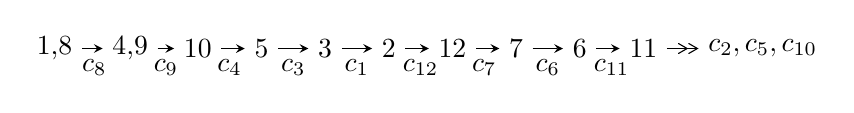
\begin{tikzpicture}[x=23pt, y=7pt]
	% node
	\node (A0) at (-1/8, 0) {1,8};
	\node (A1) at (17/16, 0) {4,9};
	\node (A2) at (17/8, 0) {10};
	\node (A3) at (25/8, 0) {5};
	\node (A4) at (33/8, 0) {3};
	\node (A5) at (41/8, 0) {2};
	\node (A6) at (49/8, 0) {12};
	\node (A7) at (57/8, 0) {7};
	\node (A8) at (65/8, 0) {6};
	\node (A9) at (73/8, 0) {11};
	\node (C1) at (1/2, -1) {$c_{8}$};
	\node (C2) at (13/8, -1) {$c_{9}$};
	\node (C3) at (21/8, -1) {$c_{4}$};
	\node (C4) at (29/8, -1) {$c_{3}$};
	\node (C5) at (37/8, -1) {$c_{1}$};
	\node (C6) at (45/8, -1) {$c_{12}$};
	\node (C7) at (53/8, -1) {$c_{7}$};
	\node (C8) at (61/8, -1) {$c_{6}$};
	\node (C9) at (69/8, -1) {$c_{11}$};
	\node (A10) at (11, 0) {$c_{2},c_{5},c_{10}$};

	% edge
	\draw[->,>=stealth]	
	(A0) edge (A1) (A1) edge (A2) (A2) edge (A3) (A3) edge (A4) (A4) edge (A5) (A5) edge (A6) (A6) edge (A7) (A7) edge (A8) (A8) edge (A9) ;
	\draw[->>,>={angle 60}]	
	(A9) edge (A10);
\end{tikzpicture} \\ 

\end{tabular} \\

\footnotetext{
The image of knot diagram is generated by the software ``\textbf{Draw programme}" developed by Andrew Bartholomew(\url{http://www.layer8.co.uk/maths/draw/index.htm\#Running-draw}), where we modified some parts for our purpose(\url{https://github.com/CATsTAILs/LinksPainter}).
}\phantom \\ \newline 
\centering \textbf{Ideals for irreducible components\footnotemark of $X_{\text{par}}$} 
 
\begin{align*}
I^u_{1}&=\langle 
-2.56312\times10^{33} u^{48}+2.83092\times10^{33} u^{47}+\cdots+7.56342\times10^{33} b+4.45246\times10^{32},\\
\phantom{I^u_{1}}&\phantom{= \langle  }-1.28759\times10^{35} u^{48}+2.69158\times10^{35} u^{47}+\cdots+1.21015\times10^{35} a+9.76615\times10^{34},\;u^{49}-2 u^{48}+\cdots- u+1\rangle \\
I^u_{2}&=\langle 
- u^5+u^3+b- u,\;u^3+a,\;u^{18}-6 u^{16}+\cdots- u-1\rangle \\
I^u_{3}&=\langle 
b+1,\;a^4-4 a^3+3 a^2+2 a+1,\;u+1\rangle \\
I^u_{4}&=\langle 
b-1,\;a^4+4 a^3+5 a^2+2 a-1,\;u-1\rangle \\
I^u_{5}&=\langle 
b+1,\;a-1,\;u+1\rangle \\
\\
\end{align*}
\raggedright * 5 irreducible components of $\dim_{\mathbb{C}}=0$, with total 76 representations.\\
\footnotetext{All coefficients of polynomials are rational numbers. But the coefficients are sometimes approximated in decimal forms when there is not enough margin.}
\newpage
\renewcommand{\arraystretch}{1}
\centering \section*{I. $I^u_{1}= \langle -2.56\times10^{33} u^{48}+2.83\times10^{33} u^{47}+\cdots+7.56\times10^{33} b+4.45\times10^{32},\;-1.29\times10^{35} u^{48}+2.69\times10^{35} u^{47}+\cdots+1.21\times10^{35} a+9.77\times10^{34},\;u^{49}-2 u^{48}+\cdots- u+1 \rangle$}
\flushleft \textbf{(i) Arc colorings}\\
\begin{tabular}{m{7pt} m{180pt} m{7pt} m{180pt} }
\flushright $a_{1}=$&$\begin{pmatrix}0\\u\end{pmatrix}$ \\
\flushright $a_{8}=$&$\begin{pmatrix}1\\0\end{pmatrix}$ \\
\flushright $a_{4}=$&$\begin{pmatrix}1.06400 u^{48}-2.22417 u^{47}+\cdots-66.3671 u-0.807022\\0.338884 u^{48}-0.374291 u^{47}+\cdots-9.12038 u-0.0588683\end{pmatrix}$ \\
\flushright $a_{9}=$&$\begin{pmatrix}1\\- u^2\end{pmatrix}$ \\
\flushright $a_{10}=$&$\begin{pmatrix}0.0728905 u^{48}+0.0869859 u^{47}+\cdots-20.9570 u-12.0327\\-0.0255946 u^{48}-0.118358 u^{47}+\cdots+0.625886 u-1.30939\end{pmatrix}$ \\
\flushright $a_{5}=$&$\begin{pmatrix}-0.437918 u^{48}+0.654552 u^{47}+\cdots+53.0608 u+0.351204\\0.194691 u^{48}-0.265650 u^{47}+\cdots+6.68311 u+0.189616\end{pmatrix}$ \\
\flushright $a_{3}=$&$\begin{pmatrix}0.998861 u^{48}-2.15004 u^{47}+\cdots-56.0865 u-0.844336\\0.314692 u^{48}-0.206403 u^{47}+\cdots-9.12938 u-0.115001\end{pmatrix}$ \\
\flushright $a_{2}=$&$\begin{pmatrix}1.24728 u^{48}-2.43234 u^{47}+\cdots-64.0218 u-0.840988\\0.0651347 u^{48}-0.0741368 u^{47}+\cdots-9.28056 u+0.0373145\end{pmatrix}$ \\
\flushright $a_{12}=$&$\begin{pmatrix}- u\\u\end{pmatrix}$ \\
\flushright $a_{7}=$&$\begin{pmatrix}- u^2+1\\u^2\end{pmatrix}$ \\
\flushright $a_{6}=$&$\begin{pmatrix}0.0588683 u^{48}+0.221147 u^{47}+\cdots-22.4060 u-9.17925\\-0.0961828 u^{48}-0.0813832 u^{47}+\cdots+0.256973 u-1.06400\end{pmatrix}$ \\
\flushright $a_{11}=$&$\begin{pmatrix}-0.471607 u^{48}+1.41230 u^{47}+\cdots-23.3549 u-5.40971\\-0.141421 u^{48}+0.0729172 u^{47}+\cdots+2.01016 u-1.08423\end{pmatrix}$\\&\end{tabular}
\flushleft \textbf{(ii) Obstruction class $= -1$}\\~\\
\flushleft \textbf{(iii) Cusp Shapes $= -0.776631 u^{48}+0.563664 u^{47}+\cdots+20.3985 u+3.27444$}\\~\\
\newpage\renewcommand{\arraystretch}{1}
\flushleft \textbf{(iv) u-Polynomials at the component}\newline \\
\begin{tabular}{m{50pt}|m{274pt}}
Crossings & \hspace{64pt}u-Polynomials at each crossing \\
\hline $$\begin{aligned}c_{1}\end{aligned}$$&$\begin{aligned}
&u^{49}+16 u^{48}+\cdots+51 u+1
\end{aligned}$\\
\hline $$\begin{aligned}c_{2},c_{6}\end{aligned}$$&$\begin{aligned}
&u^{49}-2 u^{48}+\cdots+3 u-1
\end{aligned}$\\
\hline $$\begin{aligned}c_{3},c_{4},c_{9}\end{aligned}$$&$\begin{aligned}
&u^{49}+2 u^{48}+\cdots-24 u+16
\end{aligned}$\\
\hline $$\begin{aligned}c_{5},c_{10},c_{11}\end{aligned}$$&$\begin{aligned}
&u^{49}-2 u^{48}+\cdots-2 u+2
\end{aligned}$\\
\hline $$\begin{aligned}c_{7},c_{8},c_{12}\end{aligned}$$&$\begin{aligned}
&u^{49}+2 u^{48}+\cdots- u-1
\end{aligned}$\\
\hline
\end{tabular}\\~\\
\newpage\renewcommand{\arraystretch}{1}
\flushleft \textbf{(v) Riley Polynomials at the component}\newline \\
\begin{tabular}{m{50pt}|m{274pt}}
Crossings & \hspace{64pt}Riley Polynomials at each crossing \\
\hline $$\begin{aligned}c_{1}\end{aligned}$$&$\begin{aligned}
&y^{49}+44 y^{48}+\cdots+1819 y-1
\end{aligned}$\\
\hline $$\begin{aligned}c_{2},c_{6}\end{aligned}$$&$\begin{aligned}
&y^{49}-16 y^{48}+\cdots+51 y-1
\end{aligned}$\\
\hline $$\begin{aligned}c_{3},c_{4},c_{9}\end{aligned}$$&$\begin{aligned}
&y^{49}-50 y^{48}+\cdots-8256 y-256
\end{aligned}$\\
\hline $$\begin{aligned}c_{5},c_{10},c_{11}\end{aligned}$$&$\begin{aligned}
&y^{49}+38 y^{48}+\cdots+8 y-4
\end{aligned}$\\
\hline $$\begin{aligned}c_{7},c_{8},c_{12}\end{aligned}$$&$\begin{aligned}
&y^{49}-56 y^{48}+\cdots+99 y-1
\end{aligned}$\\
\hline
\end{tabular}\\~\\
\newpage\flushleft \textbf{(vi) Complex Volumes and Cusp Shapes}
$$\begin{array}{c|c|c}  
\text{Solutions to }I^u_{1}& \I (\text{vol} + \sqrt{-1}CS) & \text{Cusp shape}\\
 \hline 
\begin{aligned}
u &= -0.506103 + 0.862902 I \\
a &= \phantom{-}0.500355 + 1.042960 I \\
b &= \phantom{-}0.781459 + 0.968591 I\end{aligned}
 & \phantom{-}3.13730 - 0.87606 I & \phantom{-}7.33623 + 1.94038 I \\ \hline\begin{aligned}
u &= -0.506103 - 0.862902 I \\
a &= \phantom{-}0.500355 - 1.042960 I \\
b &= \phantom{-}0.781459 - 0.968591 I\end{aligned}
 & \phantom{-}3.13730 + 0.87606 I & \phantom{-}7.33623 - 1.94038 I \\ \hline\begin{aligned}
u &= -0.441469 + 0.898603 I \\
a &= \phantom{-}0.587546 + 0.830187 I \\
b &= \phantom{-}1.30109 + 0.70065 I\end{aligned}
 & \phantom{-}2.66998 - 10.11010 I & \phantom{-}6.39603 + 7.85117 I \\ \hline\begin{aligned}
u &= -0.441469 - 0.898603 I \\
a &= \phantom{-}0.587546 - 0.830187 I \\
b &= \phantom{-}1.30109 - 0.70065 I\end{aligned}
 & \phantom{-}2.66998 + 10.11010 I & \phantom{-}6.39603 - 7.85117 I \\ \hline\begin{aligned}
u &= \phantom{-}0.473125 + 0.885514 I \\
a &= -0.561307 + 0.937339 I \\
b &= -1.076850 + 0.869299 I\end{aligned}
 & \phantom{-}6.86021 + 5.51403 I & \phantom{-}10.47160 - 5.14621 I \\ \hline\begin{aligned}
u &= \phantom{-}0.473125 - 0.885514 I \\
a &= -0.561307 - 0.937339 I \\
b &= -1.076850 - 0.869299 I\end{aligned}
 & \phantom{-}6.86021 - 5.51403 I & \phantom{-}10.47160 + 5.14621 I \\ \hline\begin{aligned}
u &= \phantom{-}1.06485\phantom{ +0.000000I} \\
a &= \phantom{-}1.21417\phantom{ +0.000000I} \\
b &= -0.142650\phantom{ +0.000000I}\end{aligned}
 & \phantom{-}5.55834\phantom{ +0.000000I} & \phantom{-}16.5270\phantom{ +0.000000I} \\ \hline\begin{aligned}
u &= -1.080520 + 0.079944 I \\
a &= -1.207880 + 0.284396 I \\
b &= \phantom{-}0.160341 - 0.198571 I\end{aligned}
 & \phantom{-}1.65369 - 3.96617 I & \phantom{-}11.77753 + 3.57951 I \\ \hline\begin{aligned}
u &= -1.080520 - 0.079944 I \\
a &= -1.207880 - 0.284396 I \\
b &= \phantom{-}0.160341 + 0.198571 I\end{aligned}
 & \phantom{-}1.65369 + 3.96617 I & \phantom{-}11.77753 - 3.57951 I \\ \hline\begin{aligned}
u &= \phantom{-}0.272859 + 0.717075 I \\
a &= \phantom{-}0.097380 + 0.638899 I \\
b &= -0.442768 - 0.568471 I\end{aligned}
 & -4.96406 + 6.00920 I & \phantom{-}0.78370 - 7.92298 I\\
 \hline 
 \end{array}$$\newpage$$\begin{array}{c|c|c}  
\text{Solutions to }I^u_{1}& \I (\text{vol} + \sqrt{-1}CS) & \text{Cusp shape}\\
 \hline 
\begin{aligned}
u &= \phantom{-}0.272859 - 0.717075 I \\
a &= \phantom{-}0.097380 - 0.638899 I \\
b &= -0.442768 + 0.568471 I\end{aligned}
 & -4.96406 - 6.00920 I & \phantom{-}0.78370 + 7.92298 I \\ \hline\begin{aligned}
u &= \phantom{-}0.635672 + 0.423399 I \\
a &= \phantom{-}0.152656 + 0.981747 I \\
b &= \phantom{-}0.481748 - 0.043197 I\end{aligned}
 & -1.98468 + 1.46890 I & \phantom{-}7.38226 - 4.62534 I \\ \hline\begin{aligned}
u &= \phantom{-}0.635672 - 0.423399 I \\
a &= \phantom{-}0.152656 - 0.981747 I \\
b &= \phantom{-}0.481748 + 0.043197 I\end{aligned}
 & -1.98468 - 1.46890 I & \phantom{-}7.38226 + 4.62534 I \\ \hline\begin{aligned}
u &= -0.377239 + 0.635400 I \\
a &= -0.042557 + 0.925611 I \\
b &= \phantom{-}0.106013 - 0.171567 I\end{aligned}
 & -0.22370 - 3.57957 I & \phantom{-}7.57049 + 8.69582 I \\ \hline\begin{aligned}
u &= -0.377239 - 0.635400 I \\
a &= -0.042557 - 0.925611 I \\
b &= \phantom{-}0.106013 + 0.171567 I\end{aligned}
 & -0.22370 + 3.57957 I & \phantom{-}7.57049 - 8.69582 I \\ \hline\begin{aligned}
u &= -0.629729\phantom{ +0.000000I} \\
a &= \phantom{-}0.0259489\phantom{ +0.000000I} \\
b &= -0.419260\phantom{ +0.000000I}\end{aligned}
 & \phantom{-}0.715837\phantom{ +0.000000I} & \phantom{-}14.7920\phantom{ +0.000000I} \\ \hline\begin{aligned}
u &= \phantom{-}1.367690 + 0.118584 I \\
a &= -0.083488 - 0.457258 I \\
b &= \phantom{-}0.151194 - 0.356963 I\end{aligned}
 & -1.71441 + 2.34609 I & \phantom{-0.000000 } 0 \\ \hline\begin{aligned}
u &= \phantom{-}1.367690 - 0.118584 I \\
a &= -0.083488 + 0.457258 I \\
b &= \phantom{-}0.151194 + 0.356963 I\end{aligned}
 & -1.71441 - 2.34609 I & \phantom{-0.000000 } 0 \\ \hline\begin{aligned}
u &= -1.370000 + 0.090098 I \\
a &= -1.174840 + 0.183507 I \\
b &= \phantom{-}1.076130 + 0.107236 I\end{aligned}
 & \phantom{-}2.02971 - 4.19323 I & \phantom{-0.000000 } 0 \\ \hline\begin{aligned}
u &= -1.370000 - 0.090098 I \\
a &= -1.174840 - 0.183507 I \\
b &= \phantom{-}1.076130 - 0.107236 I\end{aligned}
 & \phantom{-}2.02971 + 4.19323 I & \phantom{-0.000000 } 0\\
 \hline 
 \end{array}$$\newpage$$\begin{array}{c|c|c}  
\text{Solutions to }I^u_{1}& \I (\text{vol} + \sqrt{-1}CS) & \text{Cusp shape}\\
 \hline 
\begin{aligned}
u &= \phantom{-}1.45161 + 0.04249 I \\
a &= \phantom{-}0.952579 - 0.218245 I \\
b &= -1.17797 + 0.84568 I\end{aligned}
 & \phantom{-}6.85291 + 0.94088 I & \phantom{-0.000000 } 0 \\ \hline\begin{aligned}
u &= \phantom{-}1.45161 - 0.04249 I \\
a &= \phantom{-}0.952579 + 0.218245 I \\
b &= -1.17797 - 0.84568 I\end{aligned}
 & \phantom{-}6.85291 - 0.94088 I & \phantom{-0.000000 } 0 \\ \hline\begin{aligned}
u &= -1.43096 + 0.24886 I \\
a &= \phantom{-}1.232470 + 0.036520 I \\
b &= -1.54657 - 0.17959 I\end{aligned}
 & \phantom{-}0.52977 - 9.47056 I & \phantom{-0.000000 } 0 \\ \hline\begin{aligned}
u &= -1.43096 - 0.24886 I \\
a &= \phantom{-}1.232470 - 0.036520 I \\
b &= -1.54657 + 0.17959 I\end{aligned}
 & \phantom{-}0.52977 + 9.47056 I & \phantom{-0.000000 } 0 \\ \hline\begin{aligned}
u &= -1.46839 + 0.13155 I \\
a &= \phantom{-}0.244748 + 0.347671 I \\
b &= -0.535951 - 1.225870 I\end{aligned}
 & \phantom{-}4.54898 - 2.99003 I & \phantom{-0.000000 } 0 \\ \hline\begin{aligned}
u &= -1.46839 - 0.13155 I \\
a &= \phantom{-}0.244748 - 0.347671 I \\
b &= -0.535951 + 1.225870 I\end{aligned}
 & \phantom{-}4.54898 + 2.99003 I & \phantom{-0.000000 } 0 \\ \hline\begin{aligned}
u &= -1.48327 + 0.04934 I \\
a &= -0.376466 + 0.449946 I \\
b &= \phantom{-}0.38527 - 1.44906 I\end{aligned}
 & \phantom{-}4.87290 - 2.72445 I & \phantom{-0.000000 } 0 \\ \hline\begin{aligned}
u &= -1.48327 - 0.04934 I \\
a &= -0.376466 - 0.449946 I \\
b &= \phantom{-}0.38527 + 1.44906 I\end{aligned}
 & \phantom{-}4.87290 + 2.72445 I & \phantom{-0.000000 } 0 \\ \hline\begin{aligned}
u &= \phantom{-}1.47136 + 0.20824 I \\
a &= -0.878047 + 0.378522 I \\
b &= \phantom{-}1.42808 - 0.90342 I\end{aligned}
 & \phantom{-}5.80687 + 6.61465 I & \phantom{-0.000000 } 0 \\ \hline\begin{aligned}
u &= \phantom{-}1.47136 - 0.20824 I \\
a &= -0.878047 - 0.378522 I \\
b &= \phantom{-}1.42808 + 0.90342 I\end{aligned}
 & \phantom{-}5.80687 - 6.61465 I & \phantom{-0.000000 } 0\\
 \hline 
 \end{array}$$\newpage$$\begin{array}{c|c|c}  
\text{Solutions to }I^u_{1}& \I (\text{vol} + \sqrt{-1}CS) & \text{Cusp shape}\\
 \hline 
\begin{aligned}
u &= \phantom{-}0.315421 + 0.397601 I \\
a &= \phantom{-}0.039889 + 1.284920 I \\
b &= \phantom{-}0.405532 - 0.300525 I\end{aligned}
 & -1.36715 + 1.10974 I & \phantom{-}0.89311 - 1.51851 I \\ \hline\begin{aligned}
u &= \phantom{-}0.315421 - 0.397601 I \\
a &= \phantom{-}0.039889 - 1.284920 I \\
b &= \phantom{-}0.405532 + 0.300525 I\end{aligned}
 & -1.36715 - 1.10974 I & \phantom{-}0.89311 + 1.51851 I \\ \hline\begin{aligned}
u &= -0.094951 + 0.466215 I \\
a &= -0.95838 + 1.34005 I \\
b &= -0.572924 - 0.727360 I\end{aligned}
 & -6.38447 - 0.32683 I & -3.51715 + 0.79678 I \\ \hline\begin{aligned}
u &= -0.094951 - 0.466215 I \\
a &= -0.95838 - 1.34005 I \\
b &= -0.572924 + 0.727360 I\end{aligned}
 & -6.38447 + 0.32683 I & -3.51715 - 0.79678 I \\ \hline\begin{aligned}
u &= \phantom{-}1.52723 + 0.33642 I \\
a &= -1.97469 + 0.88742 I \\
b &= \phantom{-}3.60061 - 0.27568 I\end{aligned}
 & \phantom{-}9.0434 + 14.6216 I & \phantom{-0.000000 } 0 \\ \hline\begin{aligned}
u &= \phantom{-}1.52723 - 0.33642 I \\
a &= -1.97469 - 0.88742 I \\
b &= \phantom{-}3.60061 + 0.27568 I\end{aligned}
 & \phantom{-}9.0434 - 14.6216 I & \phantom{-0.000000 } 0 \\ \hline\begin{aligned}
u &= -1.53962 + 0.32307 I \\
a &= \phantom{-}1.85586 + 0.99438 I \\
b &= -3.59315 - 0.63275 I\end{aligned}
 & \phantom{-}13.4023 - 9.9407 I & \phantom{-0.000000 } 0 \\ \hline\begin{aligned}
u &= -1.53962 - 0.32307 I \\
a &= \phantom{-}1.85586 - 0.99438 I \\
b &= -3.59315 + 0.63275 I\end{aligned}
 & \phantom{-}13.4023 + 9.9407 I & \phantom{-0.000000 } 0 \\ \hline\begin{aligned}
u &= \phantom{-}1.54894 + 0.30323 I \\
a &= -1.67927 + 1.07256 I \\
b &= \phantom{-}3.42720 - 1.03218 I\end{aligned}
 & \phantom{-}9.85027 + 5.15212 I & \phantom{-0.000000 } 0 \\ \hline\begin{aligned}
u &= \phantom{-}1.54894 - 0.30323 I \\
a &= -1.67927 - 1.07256 I \\
b &= \phantom{-}3.42720 + 1.03218 I\end{aligned}
 & \phantom{-}9.85027 - 5.15212 I & \phantom{-0.000000 } 0\\
 \hline 
 \end{array}$$\newpage$$\begin{array}{c|c|c}  
\text{Solutions to }I^u_{1}& \I (\text{vol} + \sqrt{-1}CS) & \text{Cusp shape}\\
 \hline 
\begin{aligned}
u &= \phantom{-}1.57332 + 0.22114 I \\
a &= \phantom{-}2.12554 - 0.50767 I \\
b &= -3.82426 - 0.00661 I\end{aligned}
 & \phantom{-}11.13740 + 8.11094 I & \phantom{-0.000000 } 0 \\ \hline\begin{aligned}
u &= \phantom{-}1.57332 - 0.22114 I \\
a &= \phantom{-}2.12554 + 0.50767 I \\
b &= -3.82426 + 0.00661 I\end{aligned}
 & \phantom{-}11.13740 - 8.11094 I & \phantom{-0.000000 } 0 \\ \hline\begin{aligned}
u &= -1.58534 + 0.20019 I \\
a &= -2.05798 - 0.63877 I \\
b &= \phantom{-}3.85771 + 0.41371 I\end{aligned}
 & \phantom{-}15.3567 - 3.3643 I & \phantom{-0.000000 } 0 \\ \hline\begin{aligned}
u &= -1.58534 - 0.20019 I \\
a &= -2.05798 + 0.63877 I \\
b &= \phantom{-}3.85771 - 0.41371 I\end{aligned}
 & \phantom{-}15.3567 + 3.3643 I & \phantom{-0.000000 } 0 \\ \hline\begin{aligned}
u &= \phantom{-}1.59138 + 0.17411 I \\
a &= \phantom{-}1.93614 - 0.75434 I \\
b &= -3.71746 + 0.86616 I\end{aligned}
 & \phantom{-}11.62880 - 1.45194 I & \phantom{-0.000000 } 0 \\ \hline\begin{aligned}
u &= \phantom{-}1.59138 - 0.17411 I \\
a &= \phantom{-}1.93614 + 0.75434 I \\
b &= -3.71746 - 0.86616 I\end{aligned}
 & \phantom{-}11.62880 + 1.45194 I & \phantom{-0.000000 } 0 \\ \hline\begin{aligned}
u &= -0.121685 + 0.105182 I \\
a &= \phantom{-}6.95371 + 3.79591 I \\
b &= \phantom{-}1.189100 - 0.168206 I\end{aligned}
 & -1.63772 - 4.11971 I & \phantom{-}0.12488 + 3.37346 I \\ \hline\begin{aligned}
u &= -0.121685 - 0.105182 I \\
a &= \phantom{-}6.95371 - 3.79591 I \\
b &= \phantom{-}1.189100 + 0.168206 I\end{aligned}
 & -1.63772 + 4.11971 I & \phantom{-}0.12488 - 3.37346 I \\ \hline\begin{aligned}
u &= \phantom{-}0.106744\phantom{ +0.000000I} \\
a &= -11.6080\phantom{ +0.000000I} \\
b &= -1.16523\phantom{ +0.000000I}\end{aligned}
 & \phantom{-}2.32826\phantom{ +0.000000I} & \phantom{-}4.47140\phantom{ +0.000000I}\\
 \hline 
 \end{array}$$\newpage\newpage\renewcommand{\arraystretch}{1}
\centering \section*{II. $I^u_{2}= \langle - u^5+u^3+b- u,\;u^3+a,\;u^{18}-6 u^{16}+\cdots- u-1 \rangle$}
\flushleft \textbf{(i) Arc colorings}\\
\begin{tabular}{m{7pt} m{180pt} m{7pt} m{180pt} }
\flushright $a_{1}=$&$\begin{pmatrix}0\\u\end{pmatrix}$ \\
\flushright $a_{8}=$&$\begin{pmatrix}1\\0\end{pmatrix}$ \\
\flushright $a_{4}=$&$\begin{pmatrix}- u^3\\u^5- u^3+u\end{pmatrix}$ \\
\flushright $a_{9}=$&$\begin{pmatrix}1\\- u^2\end{pmatrix}$ \\
\flushright $a_{10}=$&$\begin{pmatrix}- u^6+u^4+1\\u^8-2 u^6+2 u^4-2 u^2\end{pmatrix}$ \\
\flushright $a_{5}=$&$\begin{pmatrix}u^9-2 u^7+u^5-2 u^3+u\\- u^{11}+3 u^9-4 u^7+5 u^5-3 u^3+u\end{pmatrix}$ \\
\flushright $a_{3}=$&$\begin{pmatrix}- u\\u\end{pmatrix}$ \\
\flushright $a_{2}=$&$\begin{pmatrix}- u^3\\u^3+u\end{pmatrix}$ \\
\flushright $a_{12}=$&$\begin{pmatrix}- u\\u\end{pmatrix}$ \\
\flushright $a_{7}=$&$\begin{pmatrix}- u^2+1\\u^2\end{pmatrix}$ \\
\flushright $a_{6}=$&$\begin{pmatrix}u^4- u^2+1\\- u^4\end{pmatrix}$ \\
\flushright $a_{11}=$&$\begin{pmatrix}u^{16}-5 u^{14}+11 u^{12}-16 u^{10}+17 u^8-14 u^6+8 u^4-2 u^2+1\\- u^{16}+4 u^{14}-6 u^{12}+6 u^{10}-4 u^8+2 u^4-2 u^2\end{pmatrix}$\\&\end{tabular}
\flushleft \textbf{(ii) Obstruction class $= -1$}\\~\\
\flushleft \textbf{(iii) Cusp Shapes $= -4 u^9+12 u^7-12 u^5+12 u^3-8 u+10$}\\~\\
\newpage\renewcommand{\arraystretch}{1}
\flushleft \textbf{(iv) u-Polynomials at the component}\newline \\
\begin{tabular}{m{50pt}|m{274pt}}
Crossings & \hspace{64pt}u-Polynomials at each crossing \\
\hline $$\begin{aligned}c_{1}\end{aligned}$$&$\begin{aligned}
&u^{18}+12 u^{17}+\cdots+5 u+1
\end{aligned}$\\
\hline $$\begin{aligned}c_{2},c_{6},c_{7}\\c_{8},c_{12}\end{aligned}$$&$\begin{aligned}
&u^{18}-6 u^{16}+\cdots+u-1
\end{aligned}$\\
\hline $$\begin{aligned}c_{3},c_{4},c_{9}\end{aligned}$$&$\begin{aligned}
&(u^6- u^5-3 u^4+2 u^3+2 u^2+u-1)^3
\end{aligned}$\\
\hline $$\begin{aligned}c_{5},c_{10},c_{11}\end{aligned}$$&$\begin{aligned}
&(u^6+u^5+3 u^4+2 u^3+2 u^2+u-1)^3
\end{aligned}$\\
\hline
\end{tabular}\\~\\
\newpage\renewcommand{\arraystretch}{1}
\flushleft \textbf{(v) Riley Polynomials at the component}\newline \\
\begin{tabular}{m{50pt}|m{274pt}}
Crossings & \hspace{64pt}Riley Polynomials at each crossing \\
\hline $$\begin{aligned}c_{1}\end{aligned}$$&$\begin{aligned}
&y^{18}-12 y^{17}+\cdots+7 y+1
\end{aligned}$\\
\hline $$\begin{aligned}c_{2},c_{6},c_{7}\\c_{8},c_{12}\end{aligned}$$&$\begin{aligned}
&y^{18}-12 y^{17}+\cdots-5 y+1
\end{aligned}$\\
\hline $$\begin{aligned}c_{3},c_{4},c_{9}\end{aligned}$$&$\begin{aligned}
&(y^6-7 y^5+17 y^4-16 y^3+6 y^2-5 y+1)^3
\end{aligned}$\\
\hline $$\begin{aligned}c_{5},c_{10},c_{11}\end{aligned}$$&$\begin{aligned}
&(y^6+5 y^5+9 y^4+4 y^3-6 y^2-5 y+1)^3
\end{aligned}$\\
\hline
\end{tabular}\\~\\
\newpage\flushleft \textbf{(vi) Complex Volumes and Cusp Shapes}
$$\begin{array}{c|c|c}  
\text{Solutions to }I^u_{2}& \I (\text{vol} + \sqrt{-1}CS) & \text{Cusp shape}\\
 \hline 
\begin{aligned}
u &= -0.672231 + 0.755934 I \\
a &= -0.848635 - 0.592839 I \\
b &= -1.019800 - 0.770263 I\end{aligned}
 & \phantom{-}3.69558 - 4.59213 I & \phantom{-}8.58114 + 3.20482 I \\ \hline\begin{aligned}
u &= -0.672231 - 0.755934 I \\
a &= -0.848635 + 0.592839 I \\
b &= -1.019800 + 0.770263 I\end{aligned}
 & \phantom{-}3.69558 + 4.59213 I & \phantom{-}8.58114 - 3.20482 I \\ \hline\begin{aligned}
u &= \phantom{-}0.945797 + 0.372369 I \\
a &= -0.452617 - 0.947657 I \\
b &= \phantom{-}0.167799 + 0.459832 I\end{aligned}
 & -2.96024 - 1.97241 I & \phantom{-}4.57572 + 3.68478 I \\ \hline\begin{aligned}
u &= \phantom{-}0.945797 - 0.372369 I \\
a &= -0.452617 + 0.947657 I \\
b &= \phantom{-}0.167799 - 0.459832 I\end{aligned}
 & -2.96024 + 1.97241 I & \phantom{-}4.57572 - 3.68478 I \\ \hline\begin{aligned}
u &= \phantom{-}0.719335 + 0.743187 I \\
a &= \phantom{-}0.819709 - 0.743187 I \\
b &= \phantom{-}0.773023 - 0.902358 I\end{aligned}
 & \phantom{-}7.66009\phantom{ +0.000000I} & \phantom{-}12.26950 + 0. I\phantom{ +0.000000I} \\ \hline\begin{aligned}
u &= \phantom{-}0.719335 - 0.743187 I \\
a &= \phantom{-}0.819709 + 0.743187 I \\
b &= \phantom{-}0.773023 + 0.902358 I\end{aligned}
 & \phantom{-}7.66009\phantom{ +0.000000I} & \phantom{-}12.26950 + 0. I\phantom{ +0.000000I} \\ \hline\begin{aligned}
u &= -0.763761 + 0.724480 I \\
a &= -0.757105 - 0.887576 I \\
b &= -0.494362 - 0.949066 I\end{aligned}
 & \phantom{-}3.69558 + 4.59213 I & \phantom{-}8.58114 - 3.20482 I \\ \hline\begin{aligned}
u &= -0.763761 - 0.724480 I \\
a &= -0.757105 + 0.887576 I \\
b &= -0.494362 + 0.949066 I\end{aligned}
 & \phantom{-}3.69558 - 4.59213 I & \phantom{-}8.58114 + 3.20482 I \\ \hline\begin{aligned}
u &= \phantom{-}1.18645\phantom{ +0.000000I} \\
a &= -1.67012\phantom{ +0.000000I} \\
b &= \phantom{-}1.86730\phantom{ +0.000000I}\end{aligned}
 & \phantom{-}0.738851\phantom{ +0.000000I} & \phantom{-}13.4170\phantom{ +0.000000I} \\ \hline\begin{aligned}
u &= -1.219960 + 0.167385 I \\
a &= \phantom{-}1.71314 - 0.74267 I \\
b &= -1.70520 + 1.20889 I\end{aligned}
 & -2.96024 - 1.97241 I & \phantom{-}4.57572 + 3.68478 I\\
 \hline 
 \end{array}$$\newpage$$\begin{array}{c|c|c}  
\text{Solutions to }I^u_{2}& \I (\text{vol} + \sqrt{-1}CS) & \text{Cusp shape}\\
 \hline 
\begin{aligned}
u &= -1.219960 - 0.167385 I \\
a &= \phantom{-}1.71314 + 0.74267 I \\
b &= -1.70520 - 1.20889 I\end{aligned}
 & -2.96024 + 1.97241 I & \phantom{-}4.57572 - 3.68478 I \\ \hline\begin{aligned}
u &= -0.593225 + 0.236109 I \\
a &= \phantom{-}0.109553 - 0.236109 I \\
b &= -0.449977 + 0.100617 I\end{aligned}
 & \phantom{-}0.738851\phantom{ +0.000000I} & \phantom{-}13.41678 + 0. I\phantom{ +0.000000I} \\ \hline\begin{aligned}
u &= -0.593225 - 0.236109 I \\
a &= \phantom{-}0.109553 + 0.236109 I \\
b &= -0.449977 - 0.100617 I\end{aligned}
 & \phantom{-}0.738851\phantom{ +0.000000I} & \phantom{-}13.41678 + 0. I\phantom{ +0.000000I} \\ \hline\begin{aligned}
u &= \phantom{-}0.274166 + 0.539754 I \\
a &= \phantom{-}0.219014 + 0.035534 I \\
b &= \phantom{-}0.551041 + 0.518149 I\end{aligned}
 & -2.96024 + 1.97241 I & \phantom{-}4.57572 - 3.68478 I \\ \hline\begin{aligned}
u &= \phantom{-}0.274166 - 0.539754 I \\
a &= \phantom{-}0.219014 - 0.035534 I \\
b &= \phantom{-}0.551041 - 0.518149 I\end{aligned}
 & -2.96024 - 1.97241 I & \phantom{-}4.57572 + 3.68478 I \\ \hline\begin{aligned}
u &= \phantom{-}1.43599 + 0.03145 I \\
a &= -2.95686 - 0.19455 I \\
b &= \phantom{-}4.55589 + 0.50499 I\end{aligned}
 & \phantom{-}3.69558 + 4.59213 I & \phantom{-}8.58114 - 3.20482 I \\ \hline\begin{aligned}
u &= \phantom{-}1.43599 - 0.03145 I \\
a &= -2.95686 + 0.19455 I \\
b &= \phantom{-}4.55589 - 0.50499 I\end{aligned}
 & \phantom{-}3.69558 - 4.59213 I & \phantom{-}8.58114 + 3.20482 I \\ \hline\begin{aligned}
u &= -1.43867\phantom{ +0.000000I} \\
a &= \phantom{-}2.97771\phantom{ +0.000000I} \\
b &= -4.62413\phantom{ +0.000000I}\end{aligned}
 & \phantom{-}7.66009\phantom{ +0.000000I} & \phantom{-}12.2690\phantom{ +0.000000I}\\
 \hline 
 \end{array}$$\newpage\newpage\renewcommand{\arraystretch}{1}
\centering \section*{III. $I^u_{3}= \langle b+1,\;a^4-4 a^3+3 a^2+2 a+1,\;u+1 \rangle$}
\flushleft \textbf{(i) Arc colorings}\\
\begin{tabular}{m{7pt} m{180pt} m{7pt} m{180pt} }
\flushright $a_{1}=$&$\begin{pmatrix}0\\-1\end{pmatrix}$ \\
\flushright $a_{8}=$&$\begin{pmatrix}1\\0\end{pmatrix}$ \\
\flushright $a_{4}=$&$\begin{pmatrix}a\\-1\end{pmatrix}$ \\
\flushright $a_{9}=$&$\begin{pmatrix}1\\-1\end{pmatrix}$ \\
\flushright $a_{10}=$&$\begin{pmatrix}- a^2+a+1\\a-2\end{pmatrix}$ \\
\flushright $a_{5}=$&$\begin{pmatrix}- a^3+2 a^2+a-1\\a^2-3 a+1\end{pmatrix}$ \\
\flushright $a_{3}=$&$\begin{pmatrix}1\\a-2\end{pmatrix}$ \\
\flushright $a_{2}=$&$\begin{pmatrix}1\\a-3\end{pmatrix}$ \\
\flushright $a_{12}=$&$\begin{pmatrix}1\\-1\end{pmatrix}$ \\
\flushright $a_{7}=$&$\begin{pmatrix}0\\1\end{pmatrix}$ \\
\flushright $a_{6}=$&$\begin{pmatrix}1\\a-2\end{pmatrix}$ \\
\flushright $a_{11}=$&$\begin{pmatrix}a^3-4 a^2+3 a+1\\- a^3+5 a^2-5 a-3\end{pmatrix}$\\&\end{tabular}
\flushleft \textbf{(ii) Obstruction class $= 1$}\\~\\
\flushleft \textbf{(iii) Cusp Shapes $= -4 a^2+8 a+8$}\\~\\
\newpage\renewcommand{\arraystretch}{1}
\flushleft \textbf{(iv) u-Polynomials at the component}\newline \\
\begin{tabular}{m{50pt}|m{274pt}}
Crossings & \hspace{64pt}u-Polynomials at each crossing \\
\hline $$\begin{aligned}c_{1},c_{2},c_{12}\end{aligned}$$&$\begin{aligned}
&(u-1)^4
\end{aligned}$\\
\hline $$\begin{aligned}c_{3},c_{4},c_{9}\end{aligned}$$&$\begin{aligned}
&u^4-3 u^2+3
\end{aligned}$\\
\hline $$\begin{aligned}c_{5},c_{10},c_{11}\end{aligned}$$&$\begin{aligned}
&u^4+3 u^2+3
\end{aligned}$\\
\hline $$\begin{aligned}c_{6},c_{7},c_{8}\end{aligned}$$&$\begin{aligned}
&(u+1)^4
\end{aligned}$\\
\hline
\end{tabular}\\~\\
\newpage\renewcommand{\arraystretch}{1}
\flushleft \textbf{(v) Riley Polynomials at the component}\newline \\
\begin{tabular}{m{50pt}|m{274pt}}
Crossings & \hspace{64pt}Riley Polynomials at each crossing \\
\hline $$\begin{aligned}c_{1},c_{2},c_{6}\\c_{7},c_{8},c_{12}\end{aligned}$$&$\begin{aligned}
&(y-1)^4
\end{aligned}$\\
\hline $$\begin{aligned}c_{3},c_{4},c_{9}\end{aligned}$$&$\begin{aligned}
&(y^2-3 y+3)^2
\end{aligned}$\\
\hline $$\begin{aligned}c_{5},c_{10},c_{11}\end{aligned}$$&$\begin{aligned}
&(y^2+3 y+3)^2
\end{aligned}$\\
\hline
\end{tabular}\\~\\
\newpage\flushleft \textbf{(vi) Complex Volumes and Cusp Shapes}
$$\begin{array}{c|c|c}  
\text{Solutions to }I^u_{3}& \I (\text{vol} + \sqrt{-1}CS) & \text{Cusp shape}\\
 \hline 
\begin{aligned}
u &= -1.00000\phantom{ +0.000000I} \\
a &= -0.271230 + 0.340625 I \\
b &= -1.00000\phantom{ +0.000000I}\end{aligned}
 & \phantom{-0.000000 } -4.05977 I & \phantom{-}6.00000 + 3.46410 I \\ \hline\begin{aligned}
u &= -1.00000\phantom{ +0.000000I} \\
a &= -0.271230 - 0.340625 I \\
b &= -1.00000\phantom{ +0.000000I}\end{aligned}
 & \phantom{-0.000000 -}4.05977 I & \phantom{-}6.00000 - 3.46410 I \\ \hline\begin{aligned}
u &= -1.00000\phantom{ +0.000000I} \\
a &= \phantom{-}2.27123 + 0.34063 I \\
b &= -1.00000\phantom{ +0.000000I}\end{aligned}
 & \phantom{-0.000000 -}4.05977 I & \phantom{-}6.00000 - 3.46410 I \\ \hline\begin{aligned}
u &= -1.00000\phantom{ +0.000000I} \\
a &= \phantom{-}2.27123 - 0.34063 I \\
b &= -1.00000\phantom{ +0.000000I}\end{aligned}
 & \phantom{-0.000000 } -4.05977 I & \phantom{-}6.00000 + 3.46410 I\\
 \hline 
 \end{array}$$\newpage\newpage\renewcommand{\arraystretch}{1}
\centering \section*{IV. $I^u_{4}= \langle b-1,\;a^4+4 a^3+5 a^2+2 a-1,\;u-1 \rangle$}
\flushleft \textbf{(i) Arc colorings}\\
\begin{tabular}{m{7pt} m{180pt} m{7pt} m{180pt} }
\flushright $a_{1}=$&$\begin{pmatrix}0\\1\end{pmatrix}$ \\
\flushright $a_{8}=$&$\begin{pmatrix}1\\0\end{pmatrix}$ \\
\flushright $a_{4}=$&$\begin{pmatrix}a\\1\end{pmatrix}$ \\
\flushright $a_{9}=$&$\begin{pmatrix}1\\-1\end{pmatrix}$ \\
\flushright $a_{10}=$&$\begin{pmatrix}- a^2- a+1\\- a-2\end{pmatrix}$ \\
\flushright $a_{5}=$&$\begin{pmatrix}- a^3-2 a^2+a+1\\- a^2-3 a-1\end{pmatrix}$ \\
\flushright $a_{3}=$&$\begin{pmatrix}-1\\a+2\end{pmatrix}$ \\
\flushright $a_{2}=$&$\begin{pmatrix}-1\\a+3\end{pmatrix}$ \\
\flushright $a_{12}=$&$\begin{pmatrix}-1\\1\end{pmatrix}$ \\
\flushright $a_{7}=$&$\begin{pmatrix}0\\1\end{pmatrix}$ \\
\flushright $a_{6}=$&$\begin{pmatrix}1\\- a-2\end{pmatrix}$ \\
\flushright $a_{11}=$&$\begin{pmatrix}- a^3-4 a^2-3 a+1\\a^3+3 a^2+a-1\end{pmatrix}$\\&\end{tabular}
\flushleft \textbf{(ii) Obstruction class $= 1$}\\~\\
\flushleft \textbf{(iii) Cusp Shapes $= 4 a^2+8 a+8$}\\~\\
\newpage\renewcommand{\arraystretch}{1}
\flushleft \textbf{(iv) u-Polynomials at the component}\newline \\
\begin{tabular}{m{50pt}|m{274pt}}
Crossings & \hspace{64pt}u-Polynomials at each crossing \\
\hline $$\begin{aligned}c_{1},c_{6},c_{7}\\c_{8}\end{aligned}$$&$\begin{aligned}
&(u-1)^4
\end{aligned}$\\
\hline $$\begin{aligned}c_{2},c_{12}\end{aligned}$$&$\begin{aligned}
&(u+1)^4
\end{aligned}$\\
\hline $$\begin{aligned}c_{3},c_{4},c_{9}\end{aligned}$$&$\begin{aligned}
&u^4- u^2-1
\end{aligned}$\\
\hline $$\begin{aligned}c_{5},c_{10},c_{11}\end{aligned}$$&$\begin{aligned}
&u^4+u^2-1
\end{aligned}$\\
\hline
\end{tabular}\\~\\
\newpage\renewcommand{\arraystretch}{1}
\flushleft \textbf{(v) Riley Polynomials at the component}\newline \\
\begin{tabular}{m{50pt}|m{274pt}}
Crossings & \hspace{64pt}Riley Polynomials at each crossing \\
\hline $$\begin{aligned}c_{1},c_{2},c_{6}\\c_{7},c_{8},c_{12}\end{aligned}$$&$\begin{aligned}
&(y-1)^4
\end{aligned}$\\
\hline $$\begin{aligned}c_{3},c_{4},c_{9}\end{aligned}$$&$\begin{aligned}
&(y^2- y-1)^2
\end{aligned}$\\
\hline $$\begin{aligned}c_{5},c_{10},c_{11}\end{aligned}$$&$\begin{aligned}
&(y^2+y-1)^2
\end{aligned}$\\
\hline
\end{tabular}\\~\\
\newpage\flushleft \textbf{(vi) Complex Volumes and Cusp Shapes}
$$\begin{array}{c|c|c}  
\text{Solutions to }I^u_{4}& \I (\text{vol} + \sqrt{-1}CS) & \text{Cusp shape}\\
 \hline 
\begin{aligned}
u &= \phantom{-}1.00000\phantom{ +0.000000I} \\
a &= -1.000000 + 0.786151 I \\
b &= \phantom{-}1.00000\phantom{ +0.000000I}\end{aligned}
 & -3.94784\phantom{ +0.000000I} & \phantom{-}1.52786 + 0. I\phantom{ +0.000000I} \\ \hline\begin{aligned}
u &= \phantom{-}1.00000\phantom{ +0.000000I} \\
a &= -1.000000 - 0.786151 I \\
b &= \phantom{-}1.00000\phantom{ +0.000000I}\end{aligned}
 & -3.94784\phantom{ +0.000000I} & \phantom{-}1.52786 + 0. I\phantom{ +0.000000I} \\ \hline\begin{aligned}
u &= \phantom{-}1.00000\phantom{ +0.000000I} \\
a &= \phantom{-}0.272020\phantom{ +0.000000I} \\
b &= \phantom{-}1.00000\phantom{ +0.000000I}\end{aligned}
 & \phantom{-}3.94784\phantom{ +0.000000I} & \phantom{-}10.4720\phantom{ +0.000000I} \\ \hline\begin{aligned}
u &= \phantom{-}1.00000\phantom{ +0.000000I} \\
a &= -2.27202\phantom{ +0.000000I} \\
b &= \phantom{-}1.00000\phantom{ +0.000000I}\end{aligned}
 & \phantom{-}3.94784\phantom{ +0.000000I} & \phantom{-}10.4720\phantom{ +0.000000I}\\
 \hline 
 \end{array}$$\newpage\newpage\renewcommand{\arraystretch}{1}
\centering \section*{V. $I^u_{5}= \langle b+1,\;a-1,\;u+1 \rangle$}
\flushleft \textbf{(i) Arc colorings}\\
\begin{tabular}{m{7pt} m{180pt} m{7pt} m{180pt} }
\flushright $a_{1}=$&$\begin{pmatrix}0\\-1\end{pmatrix}$ \\
\flushright $a_{8}=$&$\begin{pmatrix}1\\0\end{pmatrix}$ \\
\flushright $a_{4}=$&$\begin{pmatrix}1\\-1\end{pmatrix}$ \\
\flushright $a_{9}=$&$\begin{pmatrix}1\\-1\end{pmatrix}$ \\
\flushright $a_{10}=$&$\begin{pmatrix}1\\-1\end{pmatrix}$ \\
\flushright $a_{5}=$&$\begin{pmatrix}1\\-1\end{pmatrix}$ \\
\flushright $a_{3}=$&$\begin{pmatrix}1\\-1\end{pmatrix}$ \\
\flushright $a_{2}=$&$\begin{pmatrix}1\\-2\end{pmatrix}$ \\
\flushright $a_{12}=$&$\begin{pmatrix}1\\-1\end{pmatrix}$ \\
\flushright $a_{7}=$&$\begin{pmatrix}0\\1\end{pmatrix}$ \\
\flushright $a_{6}=$&$\begin{pmatrix}1\\-1\end{pmatrix}$ \\
\flushright $a_{11}=$&$\begin{pmatrix}1\\-1\end{pmatrix}$\\&\end{tabular}
\flushleft \textbf{(ii) Obstruction class $= 1$}\\~\\
\flushleft \textbf{(iii) Cusp Shapes $= 0$}\\~\\
\newpage\renewcommand{\arraystretch}{1}
\flushleft \textbf{(iv) u-Polynomials at the component}\newline \\
\begin{tabular}{m{50pt}|m{274pt}}
Crossings & \hspace{64pt}u-Polynomials at each crossing \\
\hline $$\begin{aligned}c_{1},c_{2},c_{12}\end{aligned}$$&$\begin{aligned}
&u-1
\end{aligned}$\\
\hline $$\begin{aligned}c_{3},c_{4},c_{5}\\c_{9},c_{10},c_{11}\end{aligned}$$&$\begin{aligned}
&u
\end{aligned}$\\
\hline $$\begin{aligned}c_{6},c_{7},c_{8}\end{aligned}$$&$\begin{aligned}
&u+1
\end{aligned}$\\
\hline
\end{tabular}\\~\\
\newpage\renewcommand{\arraystretch}{1}
\flushleft \textbf{(v) Riley Polynomials at the component}\newline \\
\begin{tabular}{m{50pt}|m{274pt}}
Crossings & \hspace{64pt}Riley Polynomials at each crossing \\
\hline $$\begin{aligned}c_{1},c_{2},c_{6}\\c_{7},c_{8},c_{12}\end{aligned}$$&$\begin{aligned}
&y-1
\end{aligned}$\\
\hline $$\begin{aligned}c_{3},c_{4},c_{5}\\c_{9},c_{10},c_{11}\end{aligned}$$&$\begin{aligned}
&y
\end{aligned}$\\
\hline
\end{tabular}\\~\\
\newpage\flushleft \textbf{(vi) Complex Volumes and Cusp Shapes}
$$\begin{array}{c|c|c}  
\text{Solutions to }I^u_{5}& \I (\text{vol} + \sqrt{-1}CS) & \text{Cusp shape}\\
 \hline 
\begin{aligned}
u &= -1.00000\phantom{ +0.000000I} \\
a &= \phantom{-}1.00000\phantom{ +0.000000I} \\
b &= -1.00000\phantom{ +0.000000I}\end{aligned}
 & \phantom{-0.000000 } 0 & \phantom{-0.000000 } 0\\
 \hline 
 \end{array}$$\newpage
\newpage\renewcommand{\arraystretch}{1}
\centering \section*{ VI. u-Polynomials}
\begin{tabular}{m{50pt}|m{274pt}}
Crossings & \hspace{64pt}u-Polynomials at each crossing \\
\hline $$\begin{aligned}c_{1}\end{aligned}$$&$\begin{aligned}
&((u-1)^9)(u^{18}+12 u^{17}+\cdots+5 u+1)(u^{49}+16 u^{48}+\cdots+51 u+1)
\end{aligned}$\\
\hline $$\begin{aligned}c_{2}\end{aligned}$$&$\begin{aligned}
&((u-1)^5)(u+1)^4(u^{18}-6 u^{16}+\cdots+u-1)(u^{49}-2 u^{48}+\cdots+3 u-1)
\end{aligned}$\\
\hline $$\begin{aligned}c_{3},c_{4},c_{9}\end{aligned}$$&$\begin{aligned}
&u(u^4-3 u^2+3)(u^4- u^2-1)(u^6- u^5-3 u^4+2 u^3+2 u^2+u-1)^3\\
&\cdot(u^{49}+2 u^{48}+\cdots-24 u+16)
\end{aligned}$\\
\hline $$\begin{aligned}c_{5},c_{10},c_{11}\end{aligned}$$&$\begin{aligned}
&u(u^4+u^2-1)(u^4+3 u^2+3)(u^6+u^5+3 u^4+2 u^3+2 u^2+u-1)^3\\
&\cdot(u^{49}-2 u^{48}+\cdots-2 u+2)
\end{aligned}$\\
\hline $$\begin{aligned}c_{6}\end{aligned}$$&$\begin{aligned}
&((u-1)^4)(u+1)^5(u^{18}-6 u^{16}+\cdots+u-1)(u^{49}-2 u^{48}+\cdots+3 u-1)
\end{aligned}$\\
\hline $$\begin{aligned}c_{7},c_{8}\end{aligned}$$&$\begin{aligned}
&((u-1)^4)(u+1)^5(u^{18}-6 u^{16}+\cdots+u-1)(u^{49}+2 u^{48}+\cdots- u-1)
\end{aligned}$\\
\hline $$\begin{aligned}c_{12}\end{aligned}$$&$\begin{aligned}
&((u-1)^5)(u+1)^4(u^{18}-6 u^{16}+\cdots+u-1)(u^{49}+2 u^{48}+\cdots- u-1)
\end{aligned}$\\
\hline
\end{tabular}\newpage\renewcommand{\arraystretch}{1}
\centering \section*{ VII. Riley Polynomials}
\begin{tabular}{m{50pt}|m{274pt}}
Crossings & \hspace{64pt}Riley Polynomials at each crossing \\
\hline $$\begin{aligned}c_{1}\end{aligned}$$&$\begin{aligned}
&((y-1)^9)(y^{18}-12 y^{17}+\cdots+7 y+1)(y^{49}+44 y^{48}+\cdots+1819 y-1)
\end{aligned}$\\
\hline $$\begin{aligned}c_{2},c_{6}\end{aligned}$$&$\begin{aligned}
&((y-1)^9)(y^{18}-12 y^{17}+\cdots-5 y+1)(y^{49}-16 y^{48}+\cdots+51 y-1)
\end{aligned}$\\
\hline $$\begin{aligned}c_{3},c_{4},c_{9}\end{aligned}$$&$\begin{aligned}
&y(y^2-3 y+3)^2(y^2- y-1)^2\\
&\cdot(y^6-7 y^5+17 y^4-16 y^3+6 y^2-5 y+1)^3\\
&\cdot(y^{49}-50 y^{48}+\cdots-8256 y-256)
\end{aligned}$\\
\hline $$\begin{aligned}c_{5},c_{10},c_{11}\end{aligned}$$&$\begin{aligned}
&y(y^2+y-1)^2(y^2+3 y+3)^2(y^6+5 y^5+9 y^4+4 y^3-6 y^2-5 y+1)^3\\
&\cdot(y^{49}+38 y^{48}+\cdots+8 y-4)
\end{aligned}$\\
\hline $$\begin{aligned}c_{7},c_{8},c_{12}\end{aligned}$$&$\begin{aligned}
&((y-1)^9)(y^{18}-12 y^{17}+\cdots-5 y+1)(y^{49}-56 y^{48}+\cdots+99 y-1)
\end{aligned}$\\
\hline
\end{tabular}
\vskip 2pc
\end{document}